% =========================================================
% CONFIGURACION DEL DOCUMENTO
% =========================================================
\providecommand{\main}{..}
\documentclass[../main.tex]{subfiles}

% =========================================================
% CONTENIDO
% =========================================================
\begin{document}		
\chapter{Estado del arte}
\label{cha:02_estado_del_arte}

	En base a la investigación previa fue posible definir de forma genérica los elementos principales requeridos para la configuración y puesta en marcha de un sistema de estimulación visual y registro de movimiento ocular. En la figuras \ref{fig:02_diagrama_interfaz} y \ref{fig:02_ejemplo_setup} se presenta un diagrama general de funcionamiento del sistema propuesto y una imagen de ejemplo de un \gls{setup} típico implementado.   

	\begin{figure}[H]
		\centering
		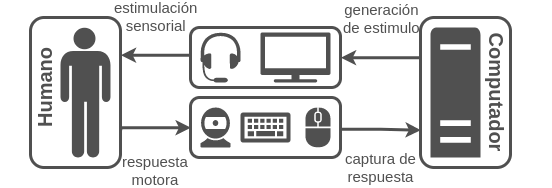
\includegraphics[width=0.7\textwidth]{cap_02_diagram}
		\caption{Diagrama general de la interfaz hombre-máquina \cite{website:baseInfo}.}
		\label{fig:02_diagrama_interfaz}
	\end{figure}

	En \ref{fig:02_diagrama_interfaz} se pretende explicitar la función del sistema de estimulación - adquisición - registro y los requerimientos del mismo. Así, el software asociado debe ser capaz de manejar la interfaz con el usuario para poder entregar estímulos (visuales principalmente) y recibir las respuestas asociadas (en forma de datos de posicionamiento ocular o respuestas solicitadas por pantalla) de forma tal de agrupar las acciones temporalmente permitiendo de esta forma dar sentido a los datos obtenidos en el experimento. 

	\newpage
	\begin{figure}[H]
		\centering
		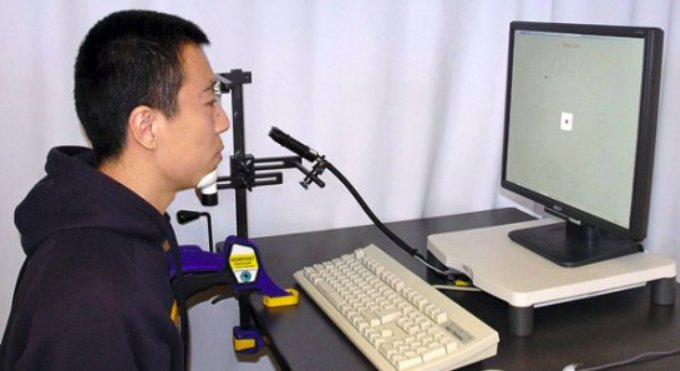
\includegraphics[width=0.5\textwidth]{cap_02_setup}
		\caption{Setup experimental típico \cite{website:baseInfo}.}
		\label{fig:02_ejemplo_setup}
	\end{figure}

	Para comprender de mejor manera el sistema y sus componentes, se presentará a modo de introducción en este capítulo una descripción de los elementos principales que forman parte del mismo. 

	\section{Sistemas de seguimiento ocular}
	\label{sec:02_sistemas_de_seguimiento_ocular}
		\subsection{Movimiento ocular}
		\label{sub:02_movimiento_ocular}

		La acción de dirigir la mirada hacia un objeto es parte fundamental del proceso de visión. Este acto involucra el direccionamiento de los \gls{ejevisual}, hacia un objetivo determinado, permitiendo la realización de análisis visuales precisos. Dicha orientación muchas veces implica movimientos coordinados de los ojos, cuello y cabeza, no obstante, existen movimientos más pequeños que son realizados únicamente por los ojos, conocidos como movimientos sacádicos \cite{article:movOcular, website:movOcular}.

		Los movimientos sacádicos corresponden a las rotaciones que realiza el globo ocular entre dos momentos de posicionamiento estacionario y que se traducen en el desplazamiento de la pupila. Estos desplazamientos pueden ocurrir tanto en el eje horizontal como vertical y cabe destacar que durante los periodos de tiempo en que se realiza el movimiento los ojos no entregan información visual relevante. Para individuos en condiciones normales este tipo de movimiento se realiza constantemente y se repite varias veces por segundo, el direccionamiento de los ojos en estos casos suele ser controlado por procesos cognitivos realizados de forma inconsciente.

		\newpage
		Las características principales de dichos movimientos son:
		\begin{enumerate}
			\item Existen dos tipos de movimientos sacádicos: Los voluntarios, también conocidos como provocados, que implican control consciente sobre los procesos cognitivos y los reflexivos o automáticos, que corresponden a la respuesta natural a la aparición de un nuevo estímulo visual.

			\item Por su naturaleza los movimientos sacádicos se consideran balísticos, lo que quiere decir que la posición de destino no cambia durante el desarrollo del movimiento. Esto puede entenderse también como que el objetivo se encuentra predeterminado en el momento de partida.

			\item La velocidad de las sacadas aumenta de forma no lineal en la medida que aumenta la amplitud de movimento y puede alcanzar magnitudes de hasta $600 - 700[\frac{deg}{s}]$. Además, la duración del movimiento puede fluctuar entre $20 - 120[ms]$, aún que en promedio solo dura de $20-40[ms]$. 

			\item La precisión del movimiento sacádico presenta un error que varía entre el $5-10\%$ de la amplitud total del movimiento. Las correcciones son realizadas por desplazamientos de calibración denominados micro-sacadas. Estos métodos correctivos permiten suponer que existe algún tipo de procesamiento paralelo encargado de la calibración ocular de largo plazo \cite{website:movOcular}.  

		\end{enumerate}

		Las características expuestas entregan, a grandes razgos, nociones que permiten comprender el por qué su estudio se ha vuelto común en campos científicos como la neurociencia: Dado que los movimientos del globo ocular son caracterizables, de patrones definidos y de alta presición es posible identificar mediante ellos enfermedades cuyos síntomas se traduzcan en alteraciones de las capacidades motrices. Un ejemplo de esto es la enfermedad de Parkinson, donde una afección crónica a los ganglios basales produce una reducción progresiva de la sustancia negra lo que se traduce en una producción insuficiente de dopamina, neurotransmisor relevante para la función motora. Esta insuficiencia se traduce en aumentos en los tiempos de respuesta y tasas de error en diversas tareas asociadas a movimiento ocular (ver \ref{sub:02_experimentos_de_estimulacion}).    

		\newpage
		\subsection{Métodos de captura}
		\label{sub:02_metodos_de_captura}
			\subsubsection{Un poco de historia} 
			\label{ssub:02_un_poco_de_historia_monitores}
			
			Para poder registrar los movimientos oculares es necesario el uso de equipamiento especializado y que, por su funcion y sin importar la tecnología utilizada, se denomina por su nombre en inglés: \gls{eyetracker}. A modo introductorio se presenta a continuación una pincelada de su desarrollo en la historia \cite{article:eyetracker_eggert, article:eyetracker_richardson}

			La primera aparición de dispositivos de este tipo data de finales del siglo XIX (Delabarre y Hale). Sus primeras versiones consistian en sistemas sumamente invasivos donde alambres finos conectados a una especie de lente de contacto movían una serie de palancas que amplificaban el movimiento y lo registraban en papel. Este método permitió objetivizar las investigaciones de comportamiento existentes. Por su contrucción, dichos dispositivos permitían observar el comportamiento espacial, más no el temporal. 

			A principios del siglo XX y de la mano de técnicas no invasivas basadas en óptica y reflexión de luz comenzaron a desarrollarse sistemas más parecidos a las tecnologías actuales: La proyección de luz sobre la córnea genera reflejos que se mueven de forma similar a la pupila y por tanto si se hace posible su registro, es posible conocer el movimiento ocular tanto horizontal como vertical, más no rotatorio (Dodge y Cline). Este método revolucionario marcaría los desarrollos futuros en esta área.

			En la década de los 70' y gracias con los avances en sistemas de grabación de video y procesamiento digital se hizo posible detectar electrónicamente características del movimiento en base al contraste existente entre la \gls{esclerotida} y los bordes del iris. Debido a los efectos de sombra producidos por los párpados este método presentaba problemas para detectar movimientos verticales, no obstante, permitía registrar movimiento horizontal con buena calidad. 

			De forma posterior y en base a estos avances iniciales fueron desarrolladas las tecnologías que, cada vez más, permiten obtener información relevante sin producir daño sobre quienes forman parte de los experimentos, reduciendo así las limitantes en este campo de investigación.    

			\subsubsection{Tecnologías actuales}
			\label{ssub:02_tecnologias_actuales}

				En la actualidad existen una gran gama de tecnologías para registrar movimiento ocular \cite{article:eyetracker_eggert, article:eyetracker_richardson, dissertation:eyetrackers}, no obstante, a continuación se indican las más relevantes: 
				\begin{enumerate}
					\item \textbf{Bobina escleral magnética (\acrshort{ssc}):} Esta técnica requiere del uso de lentes de contacto de gran tamaño directamente sobre el globo ocular. Dicho lente posee dos pequeñas bobinas de alambre que, al ser alineadas con el eje de visión, permiten obtener información sobre la dirección en la que se encuentra el ojo en forma de voltaje al ser inducidas por campos electromagnéticos externos de alta frecuencia. A pesar de la gran incomodidad que producen (ver figura \ref{fig:02_et_ssc}), esta técnica es una de las más precisas y exactas. 
					\begin{figure}[H]
						\centering
						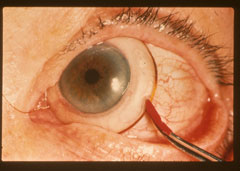
\includegraphics[width=0.35\textwidth]{cap_02_et_ssg}
						\caption{Ejemplo de uso de SSG \cite{website:etSSG}.}
						\label{fig:02_et_ssc}
					\end{figure}

					\item \textbf{Electro-OculoGrafía (\acrshort{eog}):} Esta técnica de seguimiento ocular se basa en la medición de diferencias de potencial eléctrico en la piel que se encuentra al rededor del ojo. En la medida que el ojo rota, el dipolo producido por la córnea y la retina cambia, lo que se ve reflejado en las mediciones. Sus ventajas principales, además del bajo costo, son la capacidad de medir movimiento ocular a pesar de que los ojos se encuentren cerrados, lo que hace de este método una herramienta interesante en caso de estudio de sueño y que las mediciones son relativas a la posición de la cabeza. No obstante lo anterior, la precisión y exactitud de las mediciones obtenidas es baja ya que se encuentran sujetas a artefactos como el movimiento de los párpados. La figura \ref{fig:02_et_eog} muestra el posicionamiento típico de los electrodos en este tipo de setup. 
					\begin{figure}[H]
						\centering
						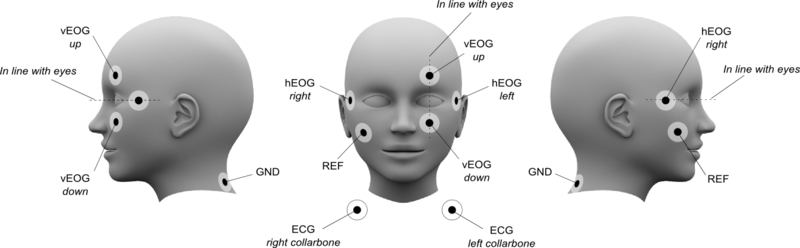
\includegraphics[width=0.9\textwidth]{cap_02_et_eog}
						\caption{Ejemplo de posicionamiento de electrodos para EOG \cite{website:etEOG}.}
						\label{fig:02_et_eog}
					\end{figure}

					\item \textbf{Seguimiento ocular basado en video (\acrshort{vog}):} Este tipo de tecnología es la más utilizada en la actualidad y corresponde a la grabación y procesamiento de la información recibida de una o más cámaras. El procesamiento puede ser dividido en dos etapas principales: en la primera se detecta y localiza el ojo en la imagen, para lo que típicamente se utiliza la pupila o el iris como punto de referencia y la segunda etapa corresponde al proceso por el cual se estima hacia donde se dirige la mirada. 

					Dentro de las técnicas VOG existentes la más popular corresponde a la detección de reflexiones de luz en la pupila y córnea. Este método suele emplear una o más cámaras y focos de luz, típicamente de tecnología infrarroja, ubicados cerca de la fuente de estimulación visual y orientados hacia el globo ocular. La tecnología infrarroja permite producir reflexiones de luz sin provocar molestia en el usuario, además de lograr evitar la mayor parte de contaminación lumínica externa. 

					El principio de funcionamiento de los métodos de reflexión se basa en las imagenes de Purkinje-Sanson que describen la existencia de al menos 4 reflexiones de luz (figura \ref{fig:02_et_vog1} (a)) que pueden ser utilizadas como referencia para estimar el direccionamiento de la pupila, como se muestra en la figura \ref{fig:02_et_vog1} (b) respecto de la primera reflexión. Además, los precios de los dispositivos que utilizan esta técnica suelen estar directamente relacionados a la cantidad o tipo de reflexiones utilizadas.
					\begin{figure}[H]
						\centering
						\subfloat[Reflexiones de Purkije-Sanson]{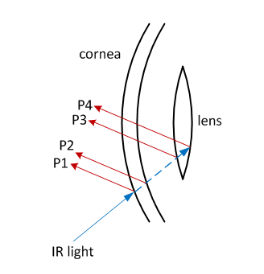
\includegraphics[width=0.3\textwidth]{cap_02_et_vog1}}\hspace{5mm}
						\subfloat[Posición de las reflexiones de la córnea (P1) relativas al centro de la pupila.]{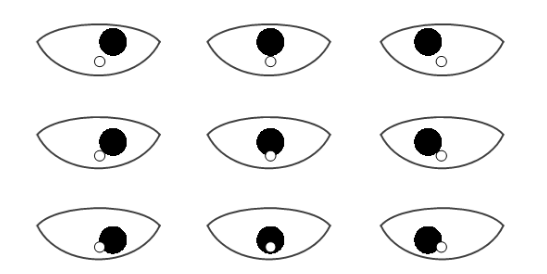
\includegraphics[width=0.55\textwidth]{cap_02_et_vog2}}
						\caption{Principio de detección VOG en base a reflexión de luz\cite{dissertation:eyetrackers}.}
						\label{fig:02_et_vog1}
					\end{figure}

					La presentación de estos dispositivos es variada y van desde cascos y lentes hasta trípodes y columnas donde se integran un elemento apoya-baribilla y el eye tracker. En la figura \ref{fig:02_et_vog2} se muestra un par a modo de referencia. 
					\begin{figure}[H]
						\centering
						\subfloat[Tobii Pro Glasses 2 \cite{website:tobii}]{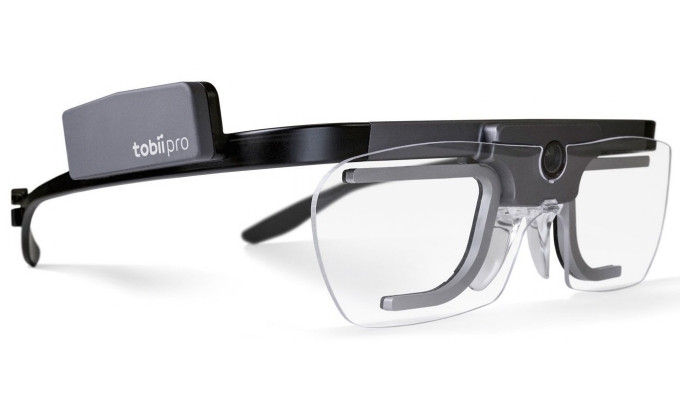
\includegraphics[width=0.4\textwidth]{cap_02_et_vog_1}}\hspace{5mm}
						\subfloat[MiraMetrix S2 \cite{website:microway}]{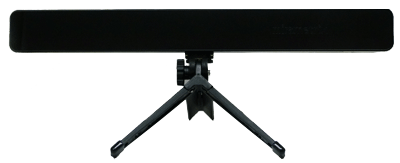
\includegraphics[width=0.4\textwidth]{cap_02_et_vog_2}}
						\caption{Muestra de eye trackers disponibles en el mercado.}
						\label{fig:02_et_vog2}
					\end{figure}  

				\end{enumerate}

			\subsubsection{Comparativa}
			\label{ssub:02_comparativa_eyetracker}

				A pesar de las claras e importantes diferencias entre las tecnologías presentadas es posible realizar una comparación entre las mismas. En \cite{article:eyetracker_eggert, article:eyetracker_richardson, dissertation:eyetrackers} se entregan nociones sobre las capacidades operativas en cuanto a presición espacial, temporal, capacidad de registrar movimientos de torsión, desplazamiento horizontal y vertical, tiempo requerido para preparar su uso (setup), comodidad para el usuario tipo de calibración requerida y complejidad de la misma. 

				En el cuadro \ref{tbl:eyetracker_compare} se presenta un resumen con las características ya descritas para EOG, SSG, VOG (común) y DPI (VOG de gama alta utilizando distintas reflexiones de Purkinje). 
				
				\begin{table}[H]\begin{center}\fontsize{10pt}{1em}{
					\singlespacing{\begin{tabular}{| C{0.18\textwidth} | C{0.18\textwidth} | C{0.18\textwidth} | C{0.18\textwidth} | C{0.18\textwidth}|}
						\hline
						 & EOG & SSG & VOG & DPI \\ \hline
						Precisión espacial (grados)	& $\approx 0.5$ & $\approx 0.01$ & $\approx 0.05$ & $\approx 0.017$\\ \hline
						Precisión temporal (Hz) 	& $40$ & $500$ & $50-400$ & $500-1000$\\ \hline
						Registro de mov. verticales	& Es posible pero se encuentran sujetos a error por efecto de artefactos producidos por el párpado & Si & Si & Si \\ \hline
						Registro de torsión			& No & Si & Si & Si \\ \hline
						Tiempo de setup				& Lento debido a que requiere la utilización de electrodos & Lento & Rápido & Rápido \\ \hline
						Requiere calibración por enfoque & Si & No & Si & Si \\ \hline
						Complejidad de calibración	& Requiere configuración bitemporal & La no-linealidad puede ser compensada con un modelo basado en ajuste de parámetros & Buena linealidad & Buena linealidad \\ \hline
						Invasividad 				& Electrodos cercanos al ojo (sin contacto), no afecta el campo visual & Lentes de contacto, posibles efectos negativos en precisión visual, incomodidad & Aparato montado en la cabeza (sin contacto con los ojos), limitación moderada del campo visual & Cabeza inmovilizada en un soporte de barbilla, limitación moderada del campo visual \\ \hline
					\end{tabular}}
					\caption{Comparativa de los sistemas de adquisición encontrados en \cite{article:eyetracker_eggert, article:eyetracker_richardson, dissertation:eyetrackers}}
					\label{tbl:eyetracker_compare}
				}\end{center}\end{table}

	\section{Sistemas de estimulación visual}
	\label{sec:02_sistemas_de_estimulacion_visual}
		\subsection{Hardware de estimulación}
		\label{sub:02_hardware_de_estimulacion}

			Para cualquier experimento científico o proyecto de investigación la reproducibilidad y repetibilidad de es tan importante como los resultados obtenidos. En este contexto, es posible aseverar que las características de los estímulos presentados son tan valiosas como el conjunto de reportes precisos sobre los parámetros utilizados para generarlos. Este motivo, en comunión con las necesidades técnicas de los experimentos, muchas veces hacen de la elección del artefacto de estimulación una tarea particularmente compleja \cite{article:monitor_beuer}.

			A lo largo de la historia, los investigadores dedicados al estudio del movimiento ocular han usado diversas tecnologías con el propósito de estimular visualmente a sus pacientes, no obstante, no fue hasta la década de los 70' y de la mano de los computadores que los monitores \acrshort{crt} revolucionaron este campo de investigación convirtiéndose en el estándar durante décadas. El motivo principal de su popularidad dice relación con la capacidad que brindan de diseñar con relativa facilidad una gran gama de pruebas y experimentos distintos, lo que permitió explorar de forma rápida nuevos métodos e hipótesis. Esto, complementado a la integración del control de los parámetros de estimulación y almacenamiento de resultados e historiales en el mismo dispositivo permitió robustecer los procesos de investigación debido a la capacidad de repetir los experimentos sin afectar mayormente características de los estímulos. 

			Las limitantes de los primeros dispositivos se fueron subsanando con el avance de la tecnología, de esta forma, los monitores análogos avanzaron hasta alcanzar tasas de refresco elevadas ($\geq 200[Hz]$), una gran gama de colores, buena resolución espacial (alcanzando hasta $1600[px]$ de ancho), un rápido decaimiento del fósforo de la pantalla que se traduce en tiempos de repuesta reducidos ($< 1[ms]$) y un buen tamaño (típicamente $20[in]$ en la diagonal). En base a esta información pueden definirse dos conceptos relevantes para el hardware de estimulación: 
			\begin{enumerate}
				\item \textbf{Tasa de refresco (\acrshort{fps}):} dice relación con la cantidad de veces que se actualiza la imagen de la pantalla por cada segundo e influye en el timing de los estímulos.
				\item \textbf{Tiempo de respuesta (\acrshort{rt}):} es cuanto demora un pixel de la pantalla en cambiar su color e influye en la calidad y nitidez de las imágenes. 
			\end{enumerate}

			A pesar de la mejoras considerables en sus características, las nuevas tecnologías han hecho desaparecer a los monitores CRT del mercado. Así en la actualidad es común ver monitores LCD, LED y oLED que tienen pantallas de mayor tamaño, menor consumo de energía, menor radiación electromagnética y una menor huella de carbono. Es importante destacar que, a pesar de que el aspecto de las nuevas tecnologías es similar, sus principios de funcionamiento, capacidades y características difieren.

			Existen varias consideraciones que hacer al utilizar estas tecnologías \cite{article:monitor_wang, article:monitor_elze}. Transversalmente se tiene un problema de timing debido a las bajas tasas de refresco de la mayor parte de los monitores modernos, por tanto en primer lugar es necesario definir los tiempos que se requiere en la muestra de frames para cumplir con los requerimientos de los estímulos. En este sentido, por ejemplo, aun que muchos monitores modernos indican que su tasa de refresco se encuentra entre $60-75[Hz]$ no se aclara en sus hojas de datos cual es el límite efectivo del refresco vertical. Este punto se vuelve crítico si se considera que una buena parte de los equipos modernos incorporan sistemas de procesamiento de imagenes para mejorar la calidad, lo que retrasa aún mas estos tiempos. Otro elemento de cuidado es el tiempo de respuesta. Es ideal asergurar que este sea reducido para lograr que el cambio entre imágenes no sea notorio y afecte el experimento (esto se hace más presente en casos en los que se muestra secuencias de video). Finalmente, es importante compaginar las características del experimento con las propiedades lumínicas del equipo ya que es sabido que en tecnologías como el caso de los LCD tanto el ángulo del observador respecto de la pantalla como las distintas zonas de la misma afectan el color/contraste observado (efecto de retro-iluminación). 
			
		\subsection{Software de estimulación}
		\label{sub:02_software_de_estimulacion}

			Tal como se indicó en el apartado anterior la generación de estímulos es una pieza clave en la realización de experimentos ya que permiten preparar un escenario adhoc para la obtención de datos específicos. En \cite{website:software} es posible encontrar una larga lista de software especializado para el desarrollo de experimentos en el área de la psicofísica además de referencias e información sobre sus características. A modo de resumen se presenta en el cuadro \ref{tbl:systems_compare} una comparación de características entre las aplicaciones más citadas de la página según google scholar.  

			\begin{table}[H]\begin{center}\fontsize{10pt}{1em}{
					\singlespacing{\begin{tabular}{| C{0.14\textwidth} | C{0.19\textwidth} | C{0.19\textwidth} | C{0.19\textwidth} | C{0.19\textwidth} |}
					\hline
					 								& PsychoPy 	& VissionEgg & PsychoToolbox & Stimulus Presentation \\\hline
					Tipo de software 				& \multicolumn{3}{c|}{Open source} & Privativo, de pago \\\hline
					Plataforma 						& \multicolumn{2}{c|}{python + OpenGL} & Matlab/Octave & Software independiente (IDE con editor de python) \\\hline
					Sistema operativo 				& \multicolumn{3}{c|}{Linux, MacOS, Windows} & Windows \\\hline
					Fecha de última actualización 	& $Dec/2017$ & $Sep/2014$ & $Oct/2017$ &  $Abr/2017$ \\\hline
					Citaciones en Google Scholar 	& $2220$ 	& $427$ 	& $6310$ 	& $3520$\\\hline
					Programable 					& \multicolumn{4}{c|}{Si}\\\hline
					Imágenes y Video 				& \multicolumn{4}{c|}{Si}\\\hline
					Sonido 							& \multicolumn{4}{c|}{Si}\\\hline
					Soporte para Eye trackers incluido 	& Si 		& No 		& Si 		& Si\\\hline
					Capacidad para registro de data 	& Si 		& No 		& Si 		& Si\\\hline
					Documentación/Foro disponible 			& Si 		& No (Link caído) & Si 	& Si\\\hline
				\end{tabular}}
				\caption{Comparativa de software de estimulación \cite{website:software_presentation, website:software_psychopy, website:software_psychotoolbox, website:software_vissionegg}}
				\label{tbl:systems_compare}
			}\end{center}\end{table}

		\newpage
		\subsection{Experimentos de estimulación}
		\label{sub:02_experimentos_de_estimulacion}

			Debido a la versatilidad de los movimientos sacádicos, se ha desarrollado con el tiempo un número importante de tareas sicomotoras para probar destintos mecanísmos cognitivos. Por este motivo y a modo de acotar las actividades asociadas a este trabajo de título, se desarrollará el sistema propuesto de forma tal que permitita solo la implementación de experimentos con características similares a los presentados en \cite{article:tests_1, article:tests_2, article:tests_3, article:tests_4}, que corresponden a métodos utilizados en la evaluación y caracterización de desempeño sicomotor en pacientes que padecen la enfermedad de Parkinson. Dichas tareas corresponden a la evaluación de movimientos pro-sacádicos, anti-sacádicos y aquellos guiados por memoria.

			En la explicación de estos experimentos se utilizarán dos elementos importantes. El primero corresponde al punto de fijación o \acrshort{fp} y el segundo al punto objetivo o \acrshort{tp}. FP es un punto ubicado en el centro de la estimulación a modo de referencia y se utiliza para calcular las amplitudes de los movimientos oculares. TP es un punto objetivo que sirve como guía en la realización de los movimientos. 

			\subsubsection{Métricas de interés}
			\label{ssub:metricas_de_interes}

				Las métricas principales a considerar para este tipo de experimentos son:
				\begin{enumerate}
				 	\item \textbf{Latencia sacádica (\acrshort{sl}):} Lapso de tiempo que transcurre entre la aparición de un nuevo estímulo y el comienzo de un movimiento de orientación en $[ms]$. 

				 	\item \textbf{Intervalo inter-sacádico (\acrshort{isi}):} Tiempo entre el término de un movimiento sacádico y el comienzo de otro en $[ms]$.
				 	
				 	\item \textbf{Ganancia inicial de movimiento:} Cociente entre la amplitud de la sacada y la distancia desde el punto de partida al objetivo. 
				 	
				 	\item \textbf{Tasa de error:} Relación entre el número de veces que el movimiento ejecutado fue errado y el total de movimientos realizados. 

				 \end{enumerate} 

			\subsubsection{Movimientos pro/anti sacádicos}
			\label{ssub:movimientos_pro_anti_sacadicos}

				A pesar de que la construcción de este tipo de tareas es sumamente similar su enfoque es completamente distinto. La medición de la respuesta prosacádica tiene como fin el cuantificar la capacidad del individuo para responder de forma reflexiva frente a un nuevo objetivo y entrega información que suele utilizarse como base para comparar otros métodos. Por otro lado, la actividad antisacádica implica la inhibición del comportamiento reflexivo y la realización de un movimiento voluntario en la dirección opuesta, de esta forma la información obtenida permite conocer el estado de estructuras cerebrales como el lóbulo frontal, en donde se procesan las funciones ejecutivas.
				\begin{figure}[H]
					\centering
					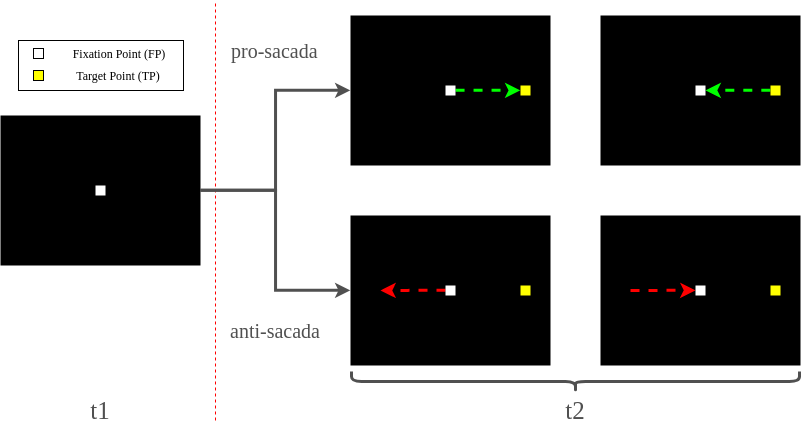
\includegraphics[width=0.8\textwidth]{cap_02_proantisaccade_base}
					\caption{Tarea pro/anti sacádica.}
					\label{fig:02_pro_anti_saccade_base}
				\end{figure}  

				Los tipos de movimientos descritos se estudian mediante estímulo similares al propuesto en la figura \ref{fig:02_pro_anti_saccade_base}. Usualmente se pide al sujeto que mantenga su vista en FP (blanco) durante algún tiempo t1 hasta que aparezca TP (amarillo) y luego realice la tarea solicitada, para lo cual se otorga un tiempo t2. En el caso de los movimientos prosacádicos, como ya fue explicado con anterioridad, se debe rotar los ojos hacia TP y luego volver a FP (flechas verdes). Para movimientos antisacádicos se realiza la acción contraria (flechas rojas). En algunos casos resulta conveniente añadir una imagen de feedback al final del experimento para indicar si la tarea fue realizada correctamente. 

				Estos experimentos pueden ser modificados y complementados con el fin de estudiar actividades cognitivas más complejas. Típicamente estas variaciones aplican uno o más de los paradigmas indicados en la figura \ref{fig:02_paradigmas}.
				\begin{figure}[H]
					\centering
					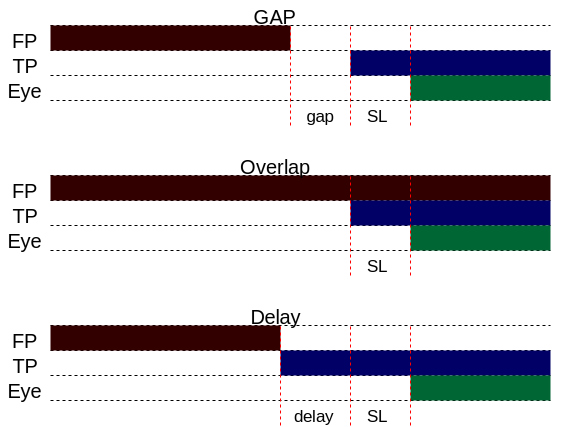
\includegraphics[width=0.5\textwidth]{cap_02_paradigmas}
					\caption{Paradigmas de experimentación.}
					\label{fig:02_paradigmas}
				\end{figure} 

			\subsubsection{Movimientos guiados por memoria}
			\label{ssub:movimientos_pro_anti_sacadicos}

				Los experimentos guiados por memoria corresponden a tareas en las cuales el usuario debe repetir con movimientos oculares algun patrón observado con anterioridad. 
				\begin{figure}[H]
					\centering
					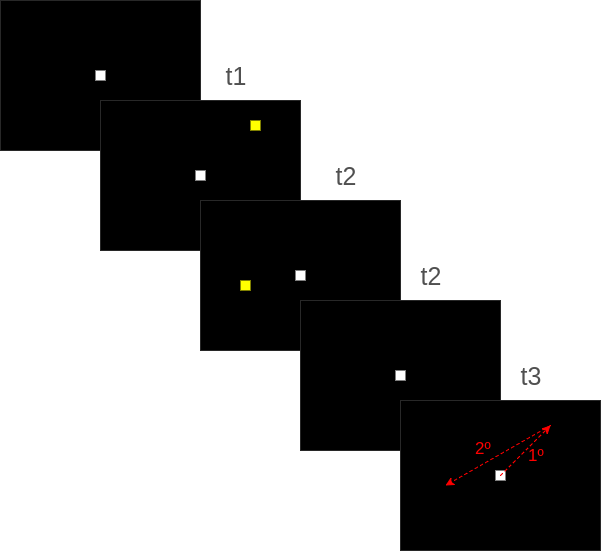
\includegraphics[width=0.7\textwidth]{cap_02_memory}
					\caption{Tarea guiada por memoria.}
					\label{fig:02_memory}
				\end{figure} 
		
				En la figura \ref{fig:02_memory} es posible observar un diseño simple para este tipo de experimentos. Despues de mantener FP por un lapso t1 en pantalla se muestra una serie de objetivos Tn en intervalos de tiempo idénticos, luego se muestra nuevamente TP por un lapso t3 para indicar que ha finalizado la serie y dar tiempo al usuario para prepararse. Finalmente se solicita que se muevan los ojos en secuencia por los puntos en que se vio aparecer los objetivos. 

\end{document}
